\section{Experiments I: the screening statistic}\label{sec:detect}

We check the statements of Section~\ref{sec:method} on the test in three steps (the deterrence and block-price laws are checked in Section~\ref{sec:policy}): with synthetic flows where the truth is known (validity, budget, power law, netting), in the agent-based market with a ring and honest groups (sensitivity, robustness, comparison with other detectors), and on real account-level order flow (Section~\ref{sec:real-accounts}). Unless stated, the agent-based results are for the default simulator (100 to 170 accounts in a window), one ring per episode, episodes of 6000 steps (19 windows of 300 steps), and the metric is \emph{catch@$B$}: the share of ring-active windows in which one of the $B$ top-ranked accounts is a ring member, with 95\% bootstrap intervals over 24 test episodes.

\subsection{Validity and the inspection budget (Propositions~\ref{prop:exact} and~\ref{prop:budget})}\label{sec:validcheck}

Figure~\ref{fig:theory}a gives the rejection rate of the implemented signed test against its nominal level for exchangeable flows. For independent Gaussian flows and for Poisson counts the rate is at the nominal level (0.0100 and 0.0102 at the 1\% level, 0.051 and 0.052 at 5\%, 18,000 tests each). Rejection is zero at the 0.1\% level because $p\ge1/T=1/300$ (Proposition~\ref{prop:budget}b). The condition of the proposition is violated by flows with a shared regime, bursts of activity that all accounts follow: the unsigned test then rejects 65\% of honest accounts at the 1\% level, and the signed test, in which symmetric bursts cancel, 1.5\%. Figure~\ref{fig:theory}b confirms the expected number of honest flags per window against the bound $N\alpha$ for $N$ from 50 to 1200, and the Bonferroni rule at level 5\% flags nothing for any of these $N$, as the resolution limit says. We therefore use the test as a ranking device and report observed rates.

\begin{figure}[t]
\centering
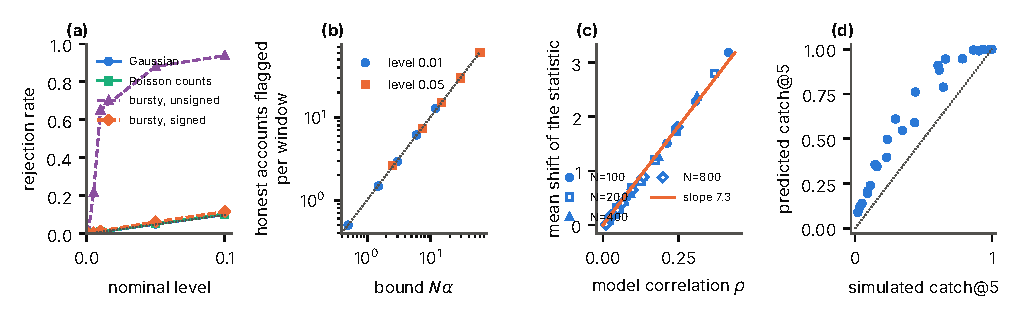
\includegraphics[width=\linewidth]{figures/theory.pdf}
\caption{Monte Carlo checks of the propositions with the implemented test. (a) Rejection rate against nominal level for exchangeable flows (Gaussian, Poisson) and for flows with a shared bursty regime (signed and unsigned variants); dotted line: nominal. (b) Honest accounts flagged per window against the bound $N\alpha$ at levels 1\% and 5\%. (c) Mean shift of a ring member's statistic against the model correlation $\rho$ of Proposition~\ref{prop:power}, for $N$ from 100 to 800, $k$ from 4 to 32 and $\eta\in\{0.1,0.3\}$; line: fitted slope. (d) Predicted against simulated catch@5 for the same 32 settings}\label{fig:theory}
\end{figure}

\subsection{The power law (Proposition~\ref{prop:power})}\label{sec:powercheck}

In a Gaussian-flow market with $N$ from 100 to 800 accounts, ring sizes from 4 to 32 and signal-to-noise ratios $\eta\in\{0.1,0.3\}$ (32 settings, 200 windows each), the mean shift of a member's statistic over the honest mean is linear in the model correlation $\rho$ of~\eqref{eq:rho} (Figure~\ref{fig:theory}c; through the origin, $R^2=0.993$; fitted slope $\sqrt{T_{\mathrm{eff}}}=7.3$, that is $T_{\mathrm{eff}}\approx53$ of $T=300$, within a factor of two of $T/(2\tau+1)=100$ for the smallest tolerance). The predicted catch@5 from~\eqref{eq:qB}, with members treated as independent, tracks the simulated one (correlation 0.96) but overstates it by 0.13 on average (Figure~\ref{fig:theory}d), because members' statistics are positively dependent through the shared signal and the shared aggregate. The law is therefore a good guide to \emph{how} detection varies with $N$ and $k$ and a poor guide to its level at small $k$.

In the agent-based market the same law explains the dependence on the number of accounts. The ring there has structure the Gaussian model omits: only the $m_{\mathrm{push}}$ members that push together are co-active, so the number of co-active accounts does not change with the ring size $K$, and the signal is proportional to the push probability. The model fitted to the three one-factor sweeps is
\begin{equation}
\text{shift}=s_0\,\frac{p_{\mathrm{push}}}{0.8}\Bigl(\frac{100}{N}\Bigr)^{1/2},\qquad
\text{catch@}B=a\,\bigl[1-(1-q_B)^K\bigr],
\label{eq:fit}
\end{equation}
with $q_B$ from~\eqref{eq:qB}, two constants ($s_0=1.20$ standard units of the statistic at $N=100$, and a ceiling $a=0.90$ for ring-active windows without signal) and the exponent $1/2$ taken from the theory. The 11 points are fitted with a mean absolute error of 0.043 (Figure~\ref{fig:powerabm}); holding one sweep out and predicting it from the other two gives errors of 0.045 for ring size, 0.085 for the number of accounts (where the $N^{-1/2}$ law is a pure prediction) and 0.088 for the push probability. When the exponent is left free it is $0.32$, below the theoretical $0.5$; with 11 points we cannot say whether this reflects the non-Gaussian flows or noise, but both give detection falling steeply with $N$: catch@5 is 0.91 at 100 accounts and 0.28 at 708.

\begin{figure}[t]
\centering
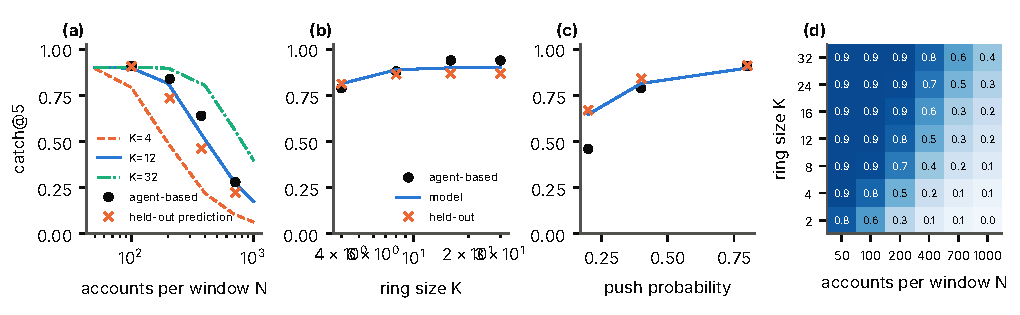
\includegraphics[width=\linewidth]{figures/power_abm.pdf}
\caption{The scaling law against the agent-based market. (a)--(c) catch@5 against the number of accounts, the ring size and the push probability: points are simulated, lines are the model~\eqref{eq:fit} fitted to all sweeps, crosses are predictions with the plotted sweep held out. (d) Model catch@5 over the number of accounts and the ring size at push probability 0.8}\label{fig:powerabm}
\end{figure}

\subsection{Honest groups and netting (Proposition~\ref{prop:netting})}\label{sec:groups}

With synthetic flows, six market-making-like desks that re-quote on both sides at the same moments are flagged at the 1\% level in 80\% of cases by the unsigned test and in 1.1\% by the signed test, whereas a one-directional ring is flagged in 37\% by the unsigned and 17\% by the signed test: netting removes the desks and costs power for the ring, as the proposition says. In the agent-based market, Table~\ref{tab:robust} and Figure~\ref{fig:robust} give catch@5 with and without honest groups. The baselines that need no labels fail on the ring: the order-to-trade ratio is dominated by market makers, which sit far above manipulators, and an isolation forest on account features finds almost nothing. The unsigned test finds the ring in a clean market but collapses when market-making desks are present, because the desks are flagged at 71\% (Table~\ref{tab:groups}) and fill the top of the ranking. Netting buys against sells removes the effect of the desks (their flag rate falls to 0 in that scenario and catch@5 stays at 0.88). A fund that splits orders across sub-accounts is genuinely coordinated and is flagged at 6\% whatever the variant; it reduces catch@5 to 0.74. With all three honest groups together catch@5 is 0.52 for the signed test and 0.23 for the unsigned one, and the desks are flagged at 18\% even after netting. A gradient-boosting model trained with labels on rings in the clean market stays at 0.98--1.00 in every scenario.

\begin{figure}[t]
\centering
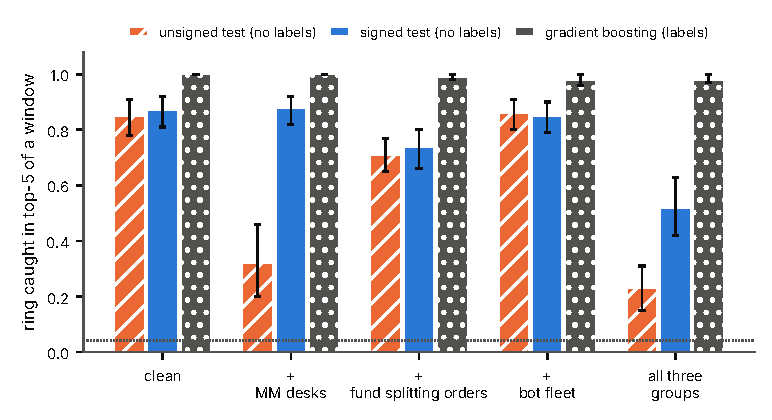
\includegraphics[width=0.85\linewidth]{figures/robust.pdf}
\caption{Share of ring-active windows in which a ring member is among the five top-ranked accounts, with 95\% bootstrap intervals over 24 episodes. The dotted line is the chance level. The unsigned test is crowded out by market-making desks; the signed test is not. Gradient boosting is trained with labels on rings in the clean market}\label{fig:robust}
\end{figure}

\begin{table}[t]
\centering\footnotesize
\adjustbox{max width=\linewidth}{\begin{tabular}{lccccc}
\toprule
detector & clean & +MM desks & +fund splitting orders & +bot fleet & all three \\
\midrule
order-to-trade ratio & 0.00\,{\scriptsize[0.00, 0.00]} & 0.00\,{\scriptsize[0.00, 0.00]} & 0.00\,{\scriptsize[0.00, 0.00]} & 0.13\,{\scriptsize[0.05, 0.22]} & 0.09\,{\scriptsize[0.04, 0.14]} \\
isolation forest (no labels) & 0.01\,{\scriptsize[0.00, 0.02]} & 0.01\,{\scriptsize[0.00, 0.02]} & 0.00\,{\scriptsize[0.00, 0.00]} & 0.01\,{\scriptsize[0.00, 0.03]} & 0.02\,{\scriptsize[0.00, 0.03]} \\
coincidence test, unsigned (no labels) & 0.85\,{\scriptsize[0.78, 0.91]} & 0.32\,{\scriptsize[0.20, 0.46]} & 0.71\,{\scriptsize[0.65, 0.77]} & 0.86\,{\scriptsize[0.80, 0.91]} & 0.23\,{\scriptsize[0.15, 0.31]} \\
coincidence test, signed (no labels) & 0.87\,{\scriptsize[0.81, 0.92]} & 0.88\,{\scriptsize[0.82, 0.92]} & 0.74\,{\scriptsize[0.66, 0.80]} & 0.85\,{\scriptsize[0.79, 0.90]} & 0.52\,{\scriptsize[0.42, 0.63]} \\
gradient boosting (labels, clean market) & 1.00\,{\scriptsize[1.00, 1.00]} & 1.00\,{\scriptsize[1.00, 1.00]} & 0.99\,{\scriptsize[0.98, 1.00]} & 0.98\,{\scriptsize[0.96, 1.00]} & 0.98\,{\scriptsize[0.97, 1.00]} \\
\bottomrule
\end{tabular}
}
\caption{catch@5 in a clean market and with honest groups acting in step (95\% bootstrap intervals).}\label{tab:robust}
\end{table}

\begin{table}[t]
\centering\footnotesize
\begin{adjustbox}{max width=\linewidth}
\begin{tabular}{llrrr}
\toprule
scenario & honest group & members scored & flagged, unsigned & flagged, signed\\
\midrule
+ market-making desks & market-making desks & 2622 & 0.711 & 0.000\\
+ fund splitting orders & fund sub-accounts & 5277 & 0.061 & 0.063\\
+ bot fleet & bot fleet & 3571 & 0.013 & 0.016\\
all three & market-making desks & 2698 & 0.665 & 0.182\\
all three & fund sub-accounts & 5202 & 0.050 & 0.053\\
all three & bot fleet & 3732 & 0.029 & 0.037\\
\bottomrule
\end{tabular}
\end{adjustbox}
\caption{Honest group members flagged at $p\le 0.01$ (nominal 1\%).}\label{tab:groups}
\end{table}

\subsection{Comparison with other detectors}\label{sec:roc}

Figure~\ref{fig:roc} gives receiver-operating and precision--recall curves of the account-window scores for the unsigned and signed tests, the supervised model and an isolation forest, in the clean market, with market-making desks and with all three honest groups. The signed test has an area under the curve of 0.85, 0.87 and 0.73 in the three scenarios and the unsigned test 0.84, 0.79 and 0.72; the supervised model 0.99, 0.99 and 0.98; the isolation forest and the order-to-trade ratio are below chance (0.36 to 0.46): the order-to-trade ratio is dominated by market makers, and the most unusual accounts by their features are not the ring members. The average precision of the label-free tests is low, 0.24, 0.27 and 0.075 for the signed test (0.22, 0.10 and 0.06 unsigned) against 0.89 to 0.94 for the supervised model and a share of 3\% to 4\% of ring members among the account-windows. The label-free tests are informative over the whole ranking but their precision is high only at its very top, which is what catch@5 measures; they are not a classifier. The netting in the signed test matters most with market-making desks (average precision 0.27 against 0.10).

\begin{figure}[t]
\centering
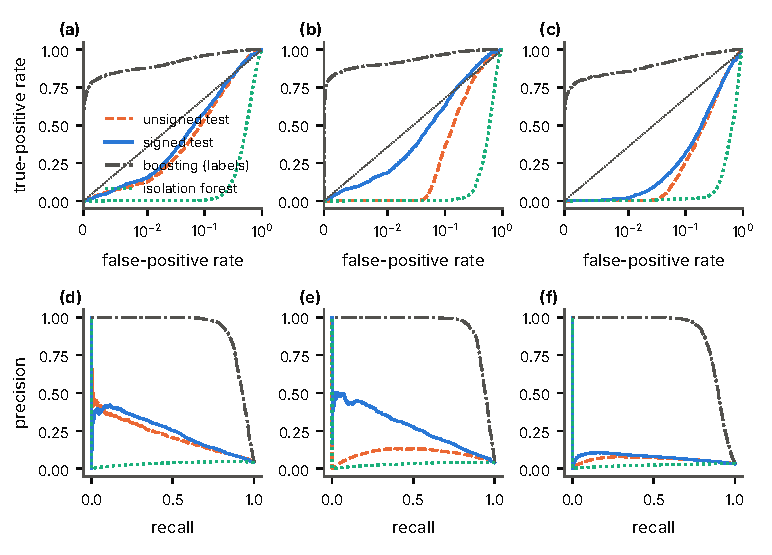
\includegraphics[width=\linewidth]{figures/roc.pdf}
\caption{Receiver-operating (top) and precision--recall (bottom) curves of account-window scores for ring membership, in a clean market (a, d), with market-making desks (b, e) and with all three honest groups (c, f); 24 test episodes each. The supervised model is trained with labels in the clean market only}\label{fig:roc}
\end{figure}

\subsection{Sensitivity}\label{sec:sens}

Figure~\ref{fig:sens} and the ablation table of Appendix~\ref{app:extra} vary the design. The tolerance set and the window length matter little (catch@5 between 0.88 and 0.91). Sensitivity falls with the number of accounts and rises with ring size (0.79 for four accounts, 0.94 for 16 or more) and with the ring's activity (0.46, 0.79, 0.91 for push probabilities 0.2, 0.4, 0.8), as the law predicts (Figure~\ref{fig:powerabm}). The dependence on the number of accounts is the main weakness of ranking by top-$B$; a rule based on finer resampling and a false-discovery-rate bound would scale differently, and we have not tested it.

\begin{figure}[t]
\centering
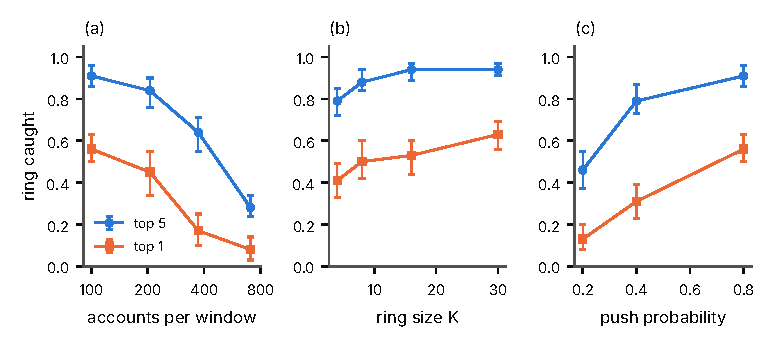
\includegraphics[width=\linewidth]{figures/sensitivity.pdf}
\caption{Sensitivity of the signed test in a clean market: (a) number of accounts per window, (b) ring size, (c) push probability of the ring. Bars are 95\% bootstrap intervals over 16 episodes}\label{fig:sens}
\end{figure}

\paragraph{What the label-free test is for.} The model trained with labels is better in every simulated scenario. The label-free test is useful when there are no labels, which is the regulator's position, and when one cannot trust that a model trained on simulated rings transfers to real ones. Section~\ref{sec:real-accounts} shows that the second concern is justified for the test itself: on real order flow it also faces a background the simulator does not contain.
